\documentclass{article}
\usepackage{hyperref}
\usepackage[margin=1in]{geometry}
\usepackage{indentfirst}   % Indents first paragraph. change if u want ig
\usepackage{setspace} 
\doublespacing
\usepackage{graphicx}
\graphicspath{ {images_arch} }
\usepackage{listings}
\usepackage{xcolor}
\usepackage{caption}
\usepackage{subcaption}
\lstset{
  basicstyle=\ttfamily,
  columns=fullflexible,
  breaklines=true,
  postbreak=\raisebox{0ex}[0ex][0ex]{\color{red}$\hookrightarrow$\space}
}

\begin{document}
\title{\textbf{Final Undergraduate Psuedo-Sudoku Submission}}
\author{Spencer Hirsch, Thomas Johnson}
\date{\today}

\maketitle

\noindent \textbf{Summary of Project}

\medskip

In our first submission we implemented a backtracking algorithm, this
algorithm worked incredibly well. However, we have now implemented a 
backtracking algorithm with a heuristic. Both of the algorithms work
in solving the test cases given, however, there is a clear difference
in the time complexities of the algorithms. 

In our intermediate submission all of our test cases were written by hand,
however, we believe that this did not challenge the algorithm enough. Therefore,
for this final submission, we have implemented a a function that generates the
test boards using randomness. Both algorithms are tested with 2700 different
test cases each. Both of our algoriths are fed the exact same test cases to better
demonstrate the time complexities of the algorithms.

In order to generate reasonable test cases to demonstrate the time complexity of 
our our two algorithms. We have implemented a generator to generate test cases to 
feed to our algorithms. Each algorithm tests a total of 2700 different test cases 
with varying difficulty. The goal of implementing a generator was to make the 
tests as random as possible and to quickly generate a more considerable sum of 
test cases. For each n (the matrix size, n x n), 15 additional test cases have 
varying m (number of missing cells). Each of these n x m combinations are tested 
30 times. This is how we have determined that 2700 different test cases are run 
on each of the algorithms. 

All aspects of the board, aside from the size of the board, are randomly determined. 
The values for each square are randomly assigned depending on board size. Once all of 
the values are determined, the number of removed cells is randomly selected and 
unique to each row. This random algorithm was created to ensure that bias was reduced. 

In order to demonstrate the time complexity of each of the algorithms, the CPU time 
is recorded for each test and plotted against the number of removed squares from 
the sudoku board. To ensure the accuracy of our results, the same test cases are 
run on both of the algorithms. Two scatter plots are constructed for the two algorithms,
one displaying every point gathered from the test sets and the other plot demonstrating
the averages of the 30 points for each n x m pair. The legend of the plots shows the total
number of cells for the test, being $n^2$. We felt that this would better visualize the size
of the test as opposed to n, the number of rows or columns.

\bigskip

\bigskip

\bigskip

\bigskip

\noindent \textbf{Backtracking Algorithm}

\begin{lstlisting}[frame=single]
	# Find next empty cell in the matrix
	def find_cell(board, size): -> int, int
		for i in range size:
			for j in range size:
				if board[i][j] is empty
					return i,j 
		return -1, -1 # Full board, return sentinal values -1, -1

	# Function checks for a valid move given the value of the current cell
	def valid_move(cord1, cord2, board, size, number): -> boolean
		# Given current cordinatess iterate through the row, and column
		# to make sure psuedo sudoku rules are not violated
		for i in range size:
			if board[i][cord2] = number 
			return false
		for j in range size:
			if board[cord1][j] = number
			return false
		return true
	
	# Implements the full back tracking algorithm
	solve(board, size): -> boolean
		nums = list(1, ... N + 1)	# stores all possible numbers
		cord1, cord2 = find_cell (board, size) # finds the next position
		if cord1 and cord2 == -1: # board is filled with legal moves
			return true
		for num cell in nums	# iterates through every possible move
			if valid_move(cord1, cord2, board, size, num):
				board[cord1][cord2] = num
				if solve(board, size):	# continue down this branch
					return true
				board[cord1][cord2] = 0	# failure, begin back tracking
		return false # could not be solved
\end{lstlisting}

\textit{How the backtracking algorithm works:} \\

\medskip
	The original algorithm is built on the idea of back tracking. To begin we first
	need to have an array storing all possible number selections for an NxN board. This means that
	if the board is 3x3 we will store the numbers [1, 2, 3] in the array \verb|nums|. The next step is to find which cell we should
	make the next valid move in, using \verb|cord1, cord2 = find_cell(board, size)|. This function works simple enough;
	it merely iterates through the rows, and columns of the inputted board to find the next blank space. 
	If no empty space is found we return the values -1, -1. This signifies the board is filled up fully, and that it is solved.

	Moving into the main bulk of the algorithm, we enumerate through each \verb|num in nums|, and use the code
	\verb|if valid_move(cord1, cord2, board, size, num)|. \verb|valid_move(...)| works on taking in the required information,
	and seeing if the current \verb|num| is a valid move at that cordinate given the ruleset of psuedo sudoko. If it is valid we return true
	else we return false, and move on to another number. If its a valid move however we set that boards cell to the current number
	\verb|board[cord1][cord2] = num|.

	Now that a valid move has been found we begin to recursively call the function using the code \verb|if solve(board, size)|. If this evaluates to true
	then the board will recursively be filled up with valid moves. However if \verb|solve(...)| evaluates to false at any point in time, the current cell is reflagged 
	as empty, and the back tracking begins. \\



\pagebreak

\noindent \textbf{Backtracking with Heuristic}

\begin{lstlisting}[frame=single]
	# Functions used prior that are unchanged:
	def find_cell(board, size) -> int, int
	def valid_move (cord1, cord2, board, size, number) -> boolean

	# New function to implement basic forward checking
	def get_unused_numbers(board, cord1, cord2, size) -> list
		nums = set of the range(1, size + 1) to hold all possible values.

		# Iterate through the row, and column of current cords to remove duplicates
		for i in range of size:
			current number = board[i][cord2]
			if current number is in nums:
				remove current number from nums
		for j in range of size:
			current number = board[cord1][j]
			if current number is in nums:
				remove current number from nums
		return list(nums)

	# This will slightly the code for solve2
	def solve2 (board, size):
		cord1, cord2 = find_cell (board, size) -> int, int
		nums = get_unused_numbers(board, cord1, cord2, size) -> list
		if cord1 and cord2 == -1:
			return true
		for num cell in nums
			if valid_move(cord1, cord2, board, size, num):
				board[cord1][cord2] = num
				if solve(board, size):
					return true
				board[cord1][cord2] = 0

\end{lstlisting}

\textit{How the backtracking with heuristic algorithm works}: \\

The only real change to the algorithm is the inclusion of the forward checking heuristic.
This is implemented by the function \verb|get_unused_numbers(...)|. This works by checking the prior moves, and
using this information to adjust which values we will attempt to use in our current move. We do this by simply taking our current list 
of numbers, iterating through the row, and column of our current cords, and then removing any numbers found during the iterations from our 
current number list.

\bigskip
\pagebreak

\noindent \textbf{Analysis of Algorithms}

\bigskip

% \noindent \textit{The lengend of the plots demonstrates the product of the size of the column and row sizes, being $n^2$. This
% was used to better showcase the true size of the test as opposed to just the size of the rows or columns of
% the board.}

% \bigskip

% \noindent \textit{Backtracking}

\bigskip

\begin{figure}[!h]
	\centering
	\begin{subfigure}{0.4\textwidth}
		\centering
		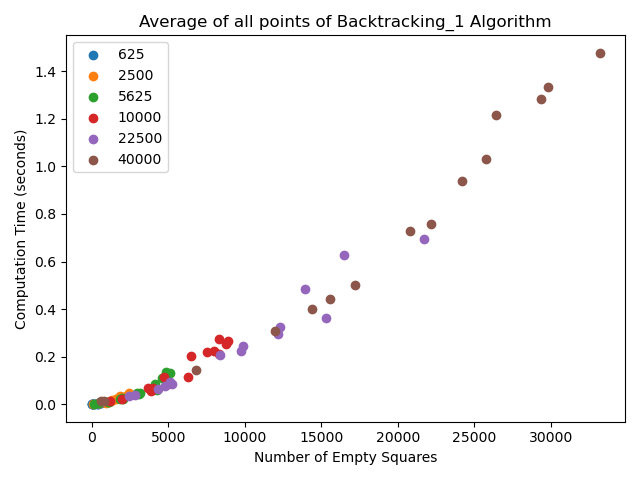
\includegraphics[scale=0.4]{scatter_avg_Backtracking_1-1.png}
		\label{Test 1: Average of all points}
		\caption{Items in the legend demonstrate the total number of cells, $n^2$}
	\end{subfigure}
	\hfill
	\begin{subfigure}{0.4\textwidth}
		\centering
		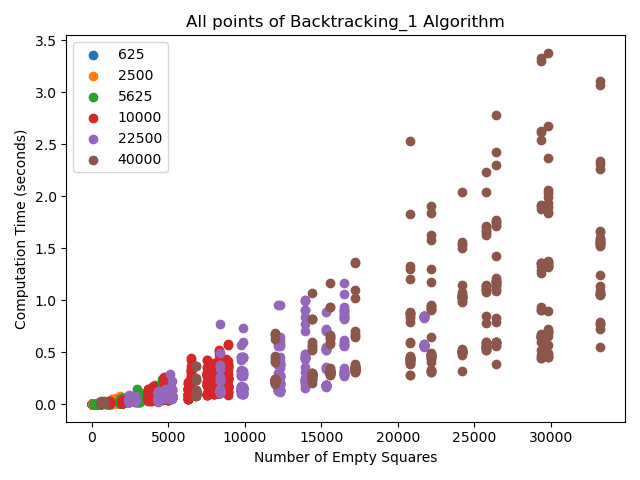
\includegraphics[scale=0.4]{scatter_Backtracking_1-1.png}
		\label{Test 1: Scatter plot of all collected points}
		\caption{Items in the legend demonstrate the total number of cells, $n^2$}
	\end{subfigure}
	\caption{Data Collected from Backtracking algorithm, Test 1.}
\end{figure}

\bigskip

% \noindent \textit{Backtracking with Heuristic} 

% \bigskip

\begin{figure}[!h]
	\centering
	\begin{subfigure}{0.4\textwidth}
		\centering
		\includegraphics[scale=0.4]{scatter_avg_Backtracking_w_Heuristic-1.png}
		\label{Test 1: Average of all points}
		\caption{Items in the legend demonstrate the total number of cells, $n^2$}
	\end{subfigure}
	\hfill
	\begin{subfigure}{0.4\textwidth}
		\centering
		\includegraphics[scale=0.4]{scatter_Backtracking_w_Heuristic-1.png}
		\label{Test 1: Scatter plot of all collected points}
		\caption{Items in the legend demonstrate the total number of cells, $n^2$}
	\end{subfigure}
	\caption{Data Collected from Backtracking algorithm with a Heuristic, Test 1.}
\end{figure}
\bigskip

From the graphs it is clear to see that there is a significant difference in
time complexity between the backtracking algorithm and the backtracking
with heuristic algorithm. \textit{Figure 1} shows what we believe to be O($n^2$) 
time complexity. As the number of missing cells increase there appears 
to be an exponential growth with respect to time. However, in the case of the backtracking algorithm with
a heuristic (\textit{Figure 2}), it is much more difficult to determine Big-Oh complexity. In this 
specific test case, Figure 2 appears to loosely conform to O(logn) complexity. However,
strictly looking at the y-axis(CPU time in seconds) on both \textit{Figure 1} and \textit{Figure 2} we can see that the backtracking 
with heuristic algorithm performs much quicker than our previous backtracking algorithm.

\bigskip

Here are some additional examples with some other test cases.

% \noindent \textit{Backtracking} 

\bigskip

\begin{figure}[!h]
	\centering
	\begin{subfigure}{0.4\textwidth}
		\centering
		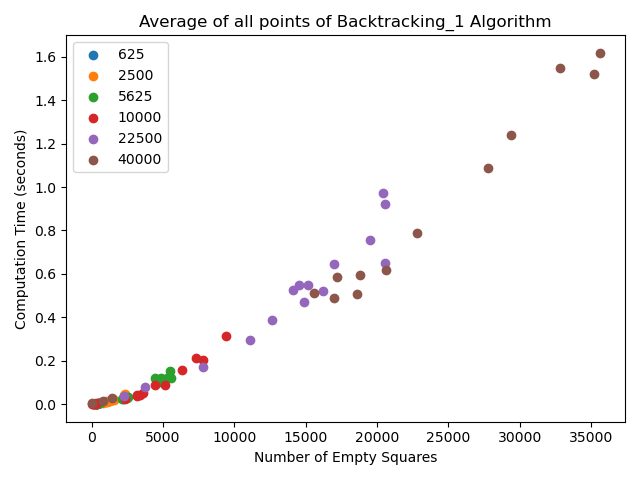
\includegraphics[scale=0.4]{scatter_avg_Backtracking_1-2.png}
		\label{Test 2: Average of all points}
		\caption{Items in the legend demonstrate the total number of cells, $n^2$}
	\end{subfigure}
	\hfill
	\begin{subfigure}{0.4\textwidth}
		\centering
		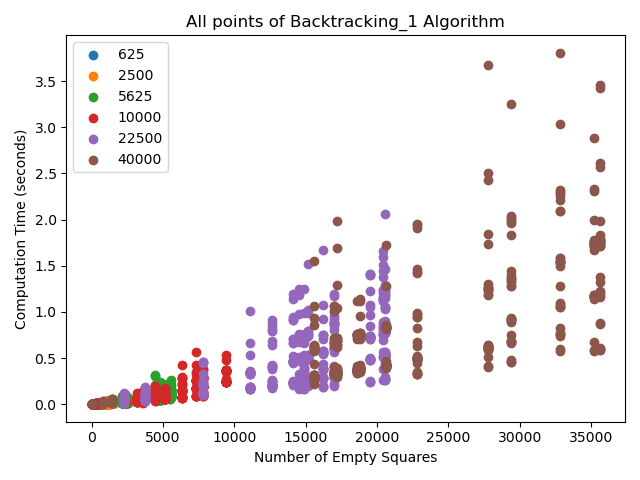
\includegraphics[scale=0.4]{scatter_Backtracking_1-2.png}
		\label{Test 2: Scatter plot of all collected points}
		\caption{Items in the legend demonstrate the total number of cells, $n^2$}
	\end{subfigure}
	\caption{Data Collected from Backtracking algorithm, Test 2.}
\end{figure}

\bigskip

% Change the images
% 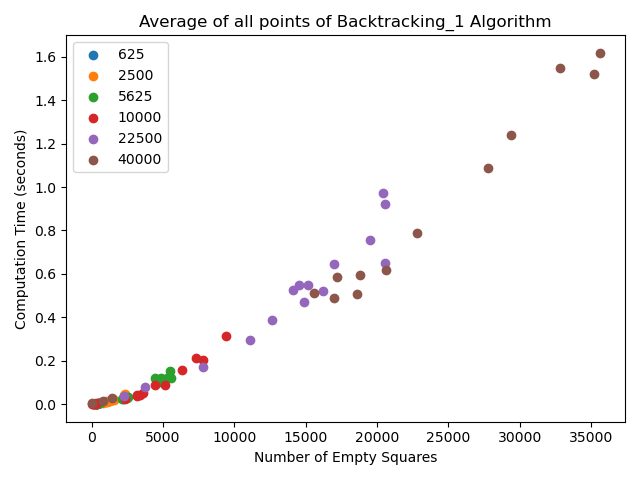
\includegraphics[scale=0.5]{scatter_avg_Backtracking_1-2.png}
% 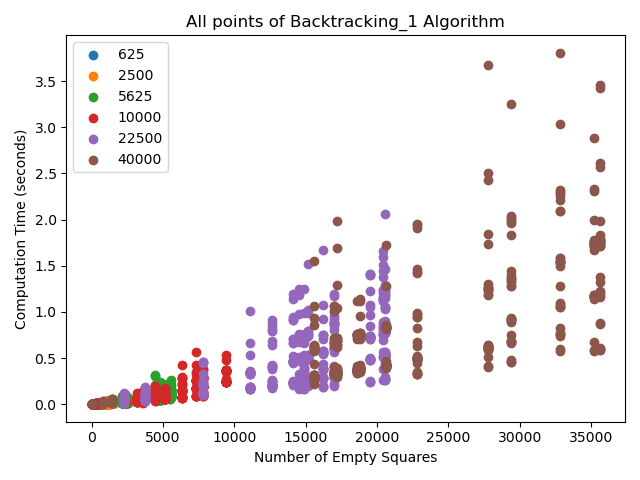
\includegraphics[scale=0.5]{scatter_Backtracking_1-2.png}

\bigskip

% \noindent \textit{Backtracking with Heuristic}

\begin{figure}[!h]
	\centering
	\begin{subfigure}{0.4\textwidth}
		\centering
		\includegraphics[scale=0.4]{scatter_avg_Backtracking_w_Heuristic-2.png}
		\label{Test 2: Average of all points}
		\caption{Items in the legend demonstrate the total number of cells, $n^2$}
	\end{subfigure}
	\hfill
	\begin{subfigure}{0.4\textwidth}
		\centering
		\includegraphics[scale=0.4]{scatter_Backtracking_w_Heuristic-2.png}
		\label{Test 2: Scatter plot of all collected points}
		\caption{Items in the legend demonstrate the total number of cells, $n^2$}
	\end{subfigure}
	\caption{Data Collected from Backtracking algorithm with a Heuristic, Test 2.}
\end{figure}
\bigskip

% Change the images
% \includegraphics[scale=0.5]{scatter_avg_Backtracking_w_Heuristic-2.png}
% \includegraphics[scale=0.5]{scatter_Backtracking_w_Heuristic-2.png}

Again, with this test case the backtracking algorithm(\textit{Figure 3}) appears to be in the shape of O($n^2$).
However, the backtracking algorithm with heuristic(\textit{Figure 4}) appears to be more in the shape of constant
time, besides the single point which is clearly an outliar. Despite the drastic change in the 
shape of the graph for the backtracking with heuristic algorithm, the backtracking with heuristic algorithm
performs much quicker than the backtracking algorithm that was originally implemented.

\bigskip

\begin{figure}[!h]
	\centering
	\begin{subfigure}{0.4\textwidth}
		\centering
		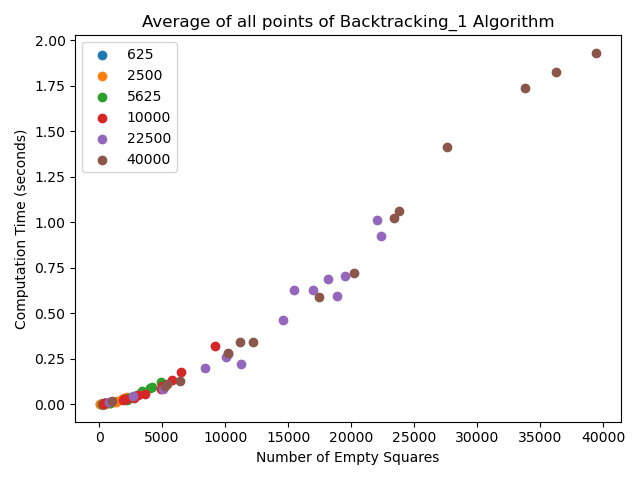
\includegraphics[scale=0.4]{scatter_avg_Backtracking_1-3.png}
		\label{Test 3: Average of all points}
		\caption{Items in the legend demonstrate the total number of cells, $n^2$}
	\end{subfigure}
	\hfill
	\begin{subfigure}{0.4\textwidth}
		\centering
		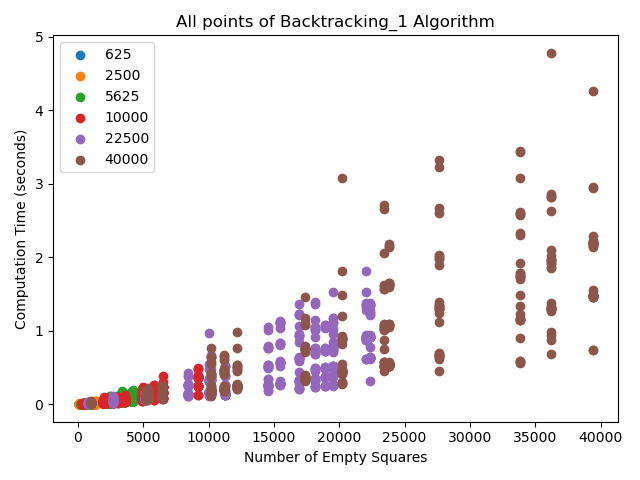
\includegraphics[scale=0.4]{scatter_Backtracking_1-3.png}
		\label{Test 3: Scatter plot of all collected points}
		\caption{Items in the legend demonstrate the total number of cells, $n^2$}
	\end{subfigure}
	\caption{Data Collected from Backtracking algorithm, Test 3.}
\end{figure}

\bigskip



% Change the images
% 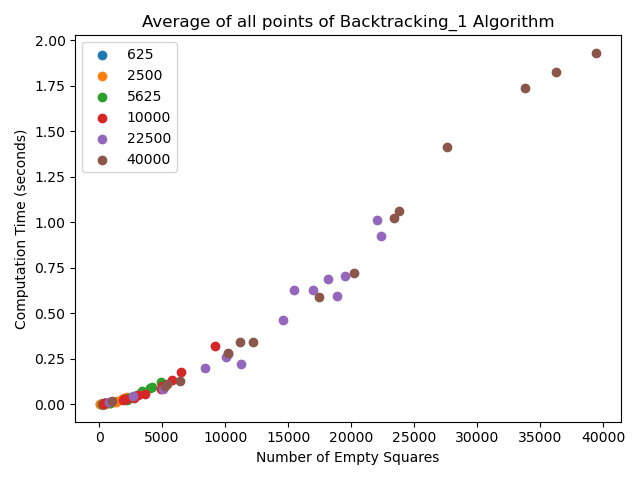
\includegraphics[scale=0.5]{scatter_avg_Backtracking_1-3.png}
% 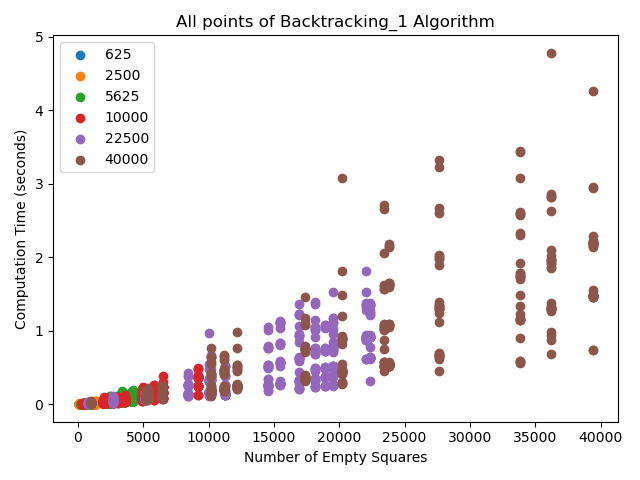
\includegraphics[scale=0.5]{scatter_Backtracking_1-3.png}

\bigskip

\begin{figure}[!h]
	\centering
	\begin{subfigure}{0.4\textwidth}
		\centering
		\includegraphics[scale=0.4]{scatter_avg_Backtracking_w_Heuristic-3.png}
		\label{Test 3: Average of all points}
		\caption{Items in the legend demonstrate the total number of cells, $n^2$}
	\end{subfigure}
	\hfill
	\begin{subfigure}{0.4\textwidth}
		\centering
		\includegraphics[scale=0.4]{scatter_Backtracking_w_Heuristic-3.png}
		\label{Test 3: Scatter plot of all collected points}
		\caption{Items in the legend demonstrate the total number of cells, $n^2$}
	\end{subfigure}
	\caption{Data Collected from Backtracking algorithm with a Heuristic, Test 3.}
\end{figure}

\bigskip


% Change the images
% \includegraphics[scale=0.5]{scatter_avg_Backtracking_w_Heuristic-3.png}
% \includegraphics[scale=0.5]{scatter_Backtracking_w_Heuristic-3.png}

These test cases aligned more with the first test case depicted in both \textit{Figure 1} and \textit{Figure 2}. The
backtracking algorithm again having more of a O($n^2$) complexity while the
backtracking with heuristic algorithm had more of a O(logn) shape. Again, 
the averages of the tests showed that the backtracking algorithm with heuristic
signigicantly outperformed the backtracking algorihtm that was originally used.

\bigskip

Overall, throughout all of the test cases that we ran on both of the algorithms. 
The newly implemented, backtracking with heuristic, significantly outperformed 
our algorithm from the first milestone submission, backtracking. Solving the problem in the 
fraction of the time. The backtracking algorithm would typically take more than a second
to solve the larger n x m problems while the backtracking with heuristic was capable of
solving it in less than 0.0002 seconds. We are very pleased and surprised with the outcome
of these results. It was very interesting to see such a drastic increase in performance 
when comparing the two algorithms and their ability to solve such large test cases. The largest
test case is a matrix of 40000 cells, a matrix 200 x 200, our backtracking with heuristic algorithm was capable
of solving it in less than 0.0002 seconds.


% \pagebreak

% \textbf{Summary of the intermediate submission:}

% \bigskip

% \noindent For this assignment, my partner and I used the backtracking algorithm in order
% to solve for the problem. Our program reads in a text file that conatins the 
% number of rows and columns as well as a list of the values that the matrix will
% be made up of. The values will be read in by row,

% \[R_{00},R_{01},R_{02},R_{03},R_{10},R_{11},R_{12},R_{13},R_{20},R_{21},R_{22},R_{23},R_{30},R_{31},R_{32},R_{33}\]

% \noindent The values are then placed in their repsective places in the n $\times$ n matrix.
% The initial empty spaces hold a value of 0, the algorithm will search for the 0's 
% in the matrix and replace them with their correct value. We chose to use a backtracking
% algorithm in order to solve this problem. The psuedo-code for our solution is posted above.
% The solution that we came to is our original code.


\end{document}